\documentclass[a4paper,12pt,twocolumn]{extarticle} \usepackage{etoolbox,fontspec,polyglossia,pdflscape,enumitem,amsfonts,amssymb,amsthm,mathtools,amsmath,icomma,euscript,mathrsfs,graphicx,wrapfig,array,tabularx,tabulary,booktabs,longtable,multirow,multicol,tikz,pdfpages}

% Настройка языка и шрифтов 
\setdefaultlanguage{russian} \setmainfont{CMU Serif} \setsansfont{CMU Sans Serif} \setmonofont{CMU Typewriter Text} \newfontfamily{\cyrillicfont}{CMU Serif} \newfontfamily{\cyrillicfontsf}{CMU Sans Serif} \newfontfamily{\cyrillicfonttt}{CMU Typewriter Text}

% Уменьшение межстрочного интервала 
\linespread{0.9}

% Уменьшение отступов абзацев 
\setlength{\parindent}{0.8em} \setlength{\parskip}{0.1em}

% Уменьшение отступов в списках 
\setlist{noitemsep,topsep=0pt,parsep=0pt,partopsep=0pt,leftmargin=0.8em}

% Уменьшение отступов вокруг формул 
\setlength{\abovedisplayskip}{3pt} \setlength{\belowdisplayskip}{3pt} \setlength{\abovedisplayshortskip}{1pt} \setlength{\belowdisplayshortskip}{1pt}

% Уменьшение отступов вокруг секций 
\usepackage{titlesec} \titlespacing{\section}{0pt}{2pt}{2pt} \titlespacing{\subsection}{0pt}{2pt}{2pt}

% Компактная геометрия страницы 
\usepackage[a4paper,landscape,left=1cm,right=1cm,top=0.8cm,bottom=0.8cm,columnsep=0.8cm,headsep=0.2cm]{geometry}

% Базовые команды и настройки 
\DeclareMathOperator{\sgn}{\mathop{sgn}} \newcommand*{\hm}[1]{#1\nobreak\discretionary{}{\hbox{$\mathsurround=0pt #1$}}{}} \graphicspath{{Изображения/}{image}} \setlength\fboxsep{2pt} \setlength\fboxrule{0.8pt}

% Настройка теорем 
\renewcommand{\thesubsection}{\arabic{subsection}} \newtheorem*{theorem}{Теорема} \newtheorem{corollary}{Следствие}
%%% Отключение колонтитулов и нумерации
\pagestyle{empty}

\begin{document}
% Неориентированные графы, cтепени, изоморфизм.
\subsection{Неориентированные графы, степени, изоморфизм}

\begin{itemize}

\item \textbf{Граф} (математическая структура для представления связей между объектами):

\begin{itemize}

\item Обозначается как $G = (X, \Gamma)$.

\item Состоит из:

\begin{enumerate}

\item[\(1^\circ\)] Непустое множество $X$ (множество всех вершин графа).

\item[\(2^\circ\)] Отображение $\Gamma$ множества $X$ в $X$ (правило, определяющее связи между вершинами).

\end{enumerate}

\end{itemize}

\item \textbf{Элементы графа}:

\begin{itemize}

\item \textbf{Вершина} (точка, узел графа): Каждый элемент множества $X$.

\item \textbf{Дуга} (направленное ребро): Пара элементов $(x, y)$, где $y \in \Gamma x$ (показывает направленную связь от $x$ к $y$).

\end{itemize}

\item \textbf{Множество дуг} (все связи в графе):

\begin{itemize}

\item Обозначается через $U$ (полный набор всех связей).

\item Дуги обозначаются буквами $\alpha$, $\beta$, $\omega$ (при необходимости с индексами).

\end{itemize}

\end{itemize}

\noindent\textbf{Определение.} Степень вершины $v_i$ (обозн. $d_i$ или $\deg v_i$) -- число рёбер, инцидентных $v_i$ (количество связей, примыкающих к вершине).

\noindent\textbf{Теорема 2.1 (Эйлера)} (фундаментальное свойство графов). Сумма степеней вершин графа равна удвоенному числу рёбер:

\[\sum_i \deg v_i = 2q\]

\noindent\textbf{Следствие 2.1(a).} Число вершин с нечётными степенями всегда чётно (важно для существования эйлеровых путей).

\noindent\textbf{Ограничения степеней:}

В $(p,q)$-графе (где $p$ -- число вершин, $q$ -- число рёбер): $0 \leq \deg v \leq p-1$ для любой вершины $v$

\noindent\textbf{Обозначения:}

\begin{itemize}

\item[$\bullet$] $\delta(G) = \min \deg G$ -- минимальная степень (наименьшее число связей у вершины)

\item[$\bullet$] $\Delta(G) = \max \deg G$ -- максимальная степень (наибольшее число связей у вершины)

\end{itemize}

\noindent\textbf{Определение.} Регулярный (однородный) граф (все вершины имеют одинаковое число связей): $\delta(G) = \Delta(G) = r = \deg G$

\noindent\textbf{Классификация регулярных графов} (по количеству связей у каждой вершины):

\begin{itemize}

\item[$\bullet$] Степень 0: граф без рёбер (изолированные точки)

\item[$\bullet$] Степень 1: компоненты -- одиночные рёбра (пары связанных вершин)

\item[$\bullet$] Степень 2: компоненты -- циклы (каждая вершина связана ровно с двумя другими)

\item[$\bullet$] Степень 3: кубические графы (каждая вершина имеет ровно три связи)

\end{itemize}

\noindent\textbf{Следствие 2.1(б).} Каждый кубический граф имеет чётное число вершин (следует из теоремы Эйлера).

\noindent\textbf{Специальные вершины:}

\begin{itemize}

\item[$\bullet$] Изолированная: $\deg v = 0$ (вершина без связей)

\item[$\bullet$] Концевая (висячая): $\deg v = 1$ (вершина с единственной связью)

\end{itemize}


% Маршруты, связность, метрика графа.
\newpage\subsection{Маршруты, связность, метрика графа}

Одно из наиболее простых свойств, которым может обладать граф, это свойство быть связным. В данном разделе рассматриваются основные структурные свойства связных и несвязных графов.
\begin{wrapfigure}{r}{0.4\textwidth}
	\centering
	\begin{tikzpicture}
		% Nodes
		\node[draw, circle, inner sep=1pt, label=below:$v_1$] (v1) at (0,0) {};
		\node[draw, circle, inner sep=1pt, label=below:$v_2$] (v2) at (2,0) {};
		\node[draw, circle, inner sep=1pt, label=below:$v_3$] (v3) at (4,0) {};
		\node[draw, circle, inner sep=1pt, label=above:$v_4$] (v4) at (1,2) {};
		\node[draw, circle, inner sep=1pt, label=above:$v_5$] (v5) at (3,2) {};
		
		% Edges
		\draw (v1) -- (v2);
		\draw (v2) -- (v3);
		\draw (v2) -- (v4);
		\draw (v2) -- (v5);
		\draw (v3) -- (v5);
		\draw (v4) -- (v5);
	\end{tikzpicture}
\end{wrapfigure}
\textit{Маршрутом} в графе $G$ называется чередующаяся последовательность вершин и рёбер $v_0, x_1, v_1, \ldots, x_n, v_n$; эта последовательность начинается и кончается вершиной, и каждое ребро последовательности инцидентно двум вершинам, одна из которых непосредственно предшествует ему, а другая непосредственно следует за ним. Указанный маршрут соединяет вершины $v_0$ и $v_n$, и его можно обозначить $v_0 v_1 v_2 \ldots v_n$ (наличие рёбер подразумевается). Эта последовательность иногда называется $(v_0-v_n)$-маршрутом. Маршрут \textit{замкнут}, если $v_0 = v_n$, и \textit{открыт} в противном случае. Маршрут называется \textit{цепью} (trail), если все его рёбра различны, и \textit{простой цепью} (path), если все вершины (а следовательно, и рёбра) различны. Замкнутая цепь называется \textit{циклом}. Замкнутый маршрут называется \textit{простым циклом}, если все его $n$ вершин различны и $n \geq 3$.

В помеченном графе $G$ на рис. 2.9 $v_1 v_2 v_3 v_2 v_3$ — маршрут, который не является цепью, а $v_1 v_2 v_5 v_4 v_2 v_3$ — не простая цепь, $v_1 v_2 v_5 v_4$ — простая цепь и $v_2 v_4 v_5 v_2$ — простой цикл.

Длина маршрута $v_0 v_1 \ldots v_n$ равна $n$, т. е. количеству рёбер в нём\footnote{Обхват графа $G$ — обозначается $g(G)$ — это длина кратчайшего простого цикла графа $G$ (если он есть); окружение графа $G$ — обозначается $c(G)$ — длина самого длинного простого цикла графа $G$. Эти понятия не определены в случае, когда в $G$ нет циклов.}.

%Самодополнительные графы
\newpage\subsection{Самодополнительные графы}

\begin{wrapfigure}{r}{0.25\textwidth}
    \begin{tikzpicture}[scale=0.8]
    % Первый граф (G)
    \begin{scope}[xshift=0cm]
        \foreach \angle [count=\i] in {90,150,...,450} {
            \node[circle, fill=black, inner sep=1.5pt] (v\i) at (\angle:1) {};
        }
        \foreach \i in {1,...,6} {
            \pgfmathtruncatemacro{\next}{mod(\i,6)+1}
            \draw (v\i) -- (v\next);
        }
        \draw (v1) -- (v4);
        \draw (v2) -- (v5);
        \draw (v3) -- (v6);
        \node at (0,-1.5) {$G$};
    \end{scope}
    
    % Второй граф (G с чертой)
    \begin{scope}[xshift=3.5cm]
        \foreach \angle [count=\i] in {30,90,...,389} {
            \node[circle, fill=black, inner sep=1.5pt] (w\i) at (\angle:1) {};
        }
        \foreach \i/\j in {1/3,3/5,5/1,2/4,4/6,6/2} {
            \draw (w\i) -- (w\j);
        }
        \node at (0,-1.5) {$\overline{G}$};
    \end{scope}
    \end{tikzpicture}
\end{wrapfigure}

\noindent\textbf{Определение.} \textit{Дополнение графа} $\overline{G}$ (граф с теми же вершинами, но противоположными связями):
\begin{itemize}[noitemsep,topsep=0pt]
\item Множество вершин: $V(\overline{G}) = V(G)$
\item Две вершины смежны в $\overline{G}$ $\Leftrightarrow$ несмежны в $G$
\end{itemize}

\noindent\textbf{Определение.} \textit{Самодополнительный граф} -- граф, изоморфный своему дополнению (структура графа совпадает со структурой его дополнения).

\noindent\textbf{Полный граф} $K_p$ (все вершины попарно соединены):
\begin{itemize}[noitemsep,topsep=0pt]
\item Содержит $p$ вершин
\item Имеет $\binom{p}{2}$ рёбер
\item Является регулярным степени $p-1$
\item Частный случай: $K_3$ -- треугольник
\end{itemize}

\noindent\textbf{Вполне несвязный граф} $\overline{K_p}$ -- дополнение полного графа (регулярный граф степени 0).

% Экстремальные графы
\newpage\subsection{Экстремальные графы}

\noindent\textbf{Теорема 2.3 (Турана)} (о максимальном числе рёбер в графе без треугольников):\\
Наибольшее число рёбер у графов с $r$ вершин без треугольников равно $\lfloor r^2/4 \rfloor$.

\noindent\textbf{Доказательство} (по индукции для чётных $r$):
\begin{enumerate}[noitemsep,topsep=0pt]
\item База: очевидна для малых $r$
\item Шаг: для $r = 2n + 2$, где утверждение верно для всех чётных $r \leq 2n$:
   \begin{itemize}[noitemsep]
   \item Пусть $G$ -- граф с $p = 2n + 2$ вершинами без треугольников
   \item Существуют смежные вершины $u$, $v$ (граф не вполне несвязный)
   \item В подграфе $G' = G - \{u, v\}$ максимум $n^2$ рёбер
   \item Нет вершины $w$, смежной с $u$ и $v$ одновременно
   \item Если $w$ смежна с $k$ вершинами $G'$, то $v$ смежна максимум с $(2n - k)$ вершинами
   \item Всего рёбер: $n^2 + k + (2n - k) + 1 = n^2 + 2n + 1 = p^2/4$
   \end{itemize}
\end{enumerate}

\noindent\textbf{Конструктивное доказательство существования:}\\
Для чётного $p$ $(p, p^2/4)$-граф без треугольников строится так:
\begin{itemize}[noitemsep]
\item Берём два множества $V_1$ и $V_2$ по $p/2$ вершин
\item Соединяем каждую вершину из $V_1$ с каждой из $V_2$
\end{itemize}

\noindent\textbf{Примечания:}
\begin{itemize}[noitemsep]
\item Доказательство существования чисел $r(m, n)$ см. у М. Холла
\item По определению бесконечный граф не является графом
\item Обзор бесконечных графов: см. Нэш-Вильямс
\end{itemize}

% Числа Рамсея
\newpage\subsection{Числа Рамсея}
Широко известна следующая головоломка.

\textit{Доказать, что среди любых шести человек найдутся либо трое попарно знакомых, либо трое попарно незнакомых.}

\begin{enumerate}
    \item Напоминаем читателю (см. введение), что в тексте не все теоремы доказываются.
    \item По своим структурным свойствам. — \textit{Прим. перев.}
\end{enumerate}

В этих терминах головоломку можно сформулировать так:

\textbf{Теорема 2.2.} Если \( G \) — граф с шестью вершинами, то либо \( G \), либо \( \overline{G} \) содержит треугольник.

\textbf{Доказательство.} Пусть \( v \) — произвольная вершина графа \( G \), имеющего шесть вершин. Так как вершина \( v \) с любой из остальных пяти вершин смежна или в \( G \), или в \( \overline{G} \), то, не теряя общности, можно предположить, что вершины \( u_1, u_2, u_3 \) смежны с \( v \) в \( G \). Если какие-либо две из вершин \( u_1, u_2, u_3 \) смежны в \( G \), то вместе с \( v \) они образуют треугольник. Если никакие две из них не смежны в \( G \), то в графе \( \overline{G} \) вершины \( u_1, u_2, u_3 \) образуют треугольник.

Обобщая теорему 2.2, естественно поставить вопрос: каково наименьшее целое число \( r(m, n) \), для которого каждый граф с \( r(m, n) \) вершинами содержит \( K_m \) или \( K_n \)?

Числа \( r(m, n) \) называются \textit{числами Рамсея} \(^1\). Ясно, что \( r(m, n) = r(n, m) \). Задача, связанная с нахождением чисел Рамсея, остается нерешенной, хотя известна простая верхняя оценка, полученная Эрдёшем и Секерешем \(^1\):

\begin{equation}
r(m, n) \leq \binom{m + n - 2}{m - 1}.
\end{equation}

Постановка этой задачи вытекает из теоремы Рамсея. Бесконечный граф \(^2\) имеет бесконечное множество вершин и не содержит кратных ребер и петель. Рамсей \(^1\) доказал (на языке теории множеств), что каждый бесконечный граф содержит \( \aleph_0 \) попарно смежных вершин или \( \aleph_0 \) попарно несмежных вершин.

Все известные числа Рамсея приведены в табл. 2.1 (взята из обзорной статьи Гравера и Якелл \(^1\)).

% Эйлеровы графы
\newpage\textbf{Эйлеровы графы}

\noindent\textbf{Эйлеров граф} -- граф, содержащий цикл со всеми вершинами и рёбрами (имеет эйлеров цикл). Обязательно связный.

\noindent\textbf{Теорема 7.1} (критерий эйлеровости). Для связного графа $G$ эквивалентны:
\begin{enumerate}
\item $G$ -- эйлеров граф
\item Все вершины имеют чётную степень
\item Рёбра можно разбить на простые циклы
\end{enumerate}

\noindent\textbf{Доказательство:}\\
(1)$\Rightarrow$(2): В эйлеровом цикле каждое прохождение вершины даёт +2 к её степени. Каждое ребро используется один раз $\Rightarrow$ степени чётны.

\noindent(2)$\Rightarrow$(3): В связном графе с чётными степенями:
\begin{itemize}[noitemsep]
\item Найдём простой цикл $Z$
\item Удалим его рёбра -- получим граф $G_1$ с чётными степенями
\item Повторяем до пустого графа $G_n$
\end{itemize}

\noindent(3)$\Rightarrow$(1): Имея разбиение на циклы:
\begin{itemize}[noitemsep]
\item Берём цикл $Z_1$
\item Находим цикл $Z_2$ с общей вершиной $v$
\item Строим замкнутую цепь из $Z_1$ и $Z_2$
\item Продолжаем до полного эйлерова цикла
\end{itemize}

\noindent\textbf{Следствие 7.1(a).} В связном графе с $2n$ вершинами нечётной степени ($n \geq 1$) рёбра можно разбить на $n$ открытых цепей.

\noindent\textbf{Следствие 7.1(б).} В связном графе с двумя вершинами нечётной степени существует открытая цепь, содержащая все рёбра (начинается и заканчивается в вершинах нечётной степени).

%Деревья
\newpage\textbf{Деревья}

\noindent\textbf{Основные определения:}
\noindent\textbf{Ациклический граф} -- граф без циклов.
\noindent\textbf{Дерево} -- связный ациклический граф.
\noindent\textbf{Лес} -- граф без циклов (компоненты -- деревья).

\noindent\textbf{Теорема 4.1.} Для графа $G$ эквивалентны:
\noindent 1) $G$ -- дерево
\noindent 2) любые две вершины соединены единственной простой цепью
\noindent 3) $G$ связен и $p = q + 1$
\noindent 4) $G$ ациклический и $p = q + 1$
\noindent 5) $G$ ациклический, и добавление любого ребра создаёт ровно один цикл
\noindent 6) $G$ связный, не $K_p$ при $p \geq 3$, добавление ребра создаёт один цикл
\noindent 7) $G$ не $K_3 \cup K_1$ и не $K_3 \cup K_2$, $p = q + 1$, добавление ребра создаёт один цикл

\noindent\textbf{Доказательство} (схема):
\noindent 1$\Rightarrow$2: От противного: две цепи образуют цикл
\noindent 2$\Rightarrow$3: Индукция по числу вершин
\noindent 3$\Rightarrow$4: От противного: цикл длины $n$ требует $q \geq p$
\noindent 4$\Rightarrow$5: Единственность компоненты из $p = q + k$
\noindent 5$\Rightarrow$6: $K_p$ при $p \geq 3$ содержит цикл
\noindent 6$\Rightarrow$7: Анализ возможных циклов
\noindent 7$\Rightarrow$1: Исключение случаев с циклами

\noindent\textbf{Следствие 4.1(а).} В нетривиальном дереве есть минимум две висячие вершины.
\noindent\textit{Доказательство:} Из $\sum d_i = 2(p-1)$ в дереве.

%Диаметр и радиус графа
\newpage\subsection{Диаметр и радиус графа}

\noindent\textbf{Расстояние} $d(u,v)$ между вершинами (длина кратчайшей простой цепи):
\[
d(u,v) = \begin{cases} 
\text{длина кратчайшей }(u\text{-}v)\text{-цепи}, & \text{если вершины соединены} \\
\infty, & \text{если вершины не соединены}
\end{cases}
\]

\noindent\textbf{Свойства метрики} (для связного графа):
\begin{enumerate}[noitemsep,topsep=0pt]
    \item $d(u,v) \geq 0$; $d(u,v) = 0 \Leftrightarrow u = v$ (неотрицательность)
    \item $d(u,v) = d(v,u)$ (симметричность)
    \item $d(u,v) + d(v,w) \geq d(u,w)$ (неравенство треугольника)
\end{enumerate}

\noindent\textbf{Термины:}
\begin{itemize}[noitemsep,topsep=0pt]
    \item \textit{Геодезическая} -- кратчайшая простая $(u\text{-}v)$-цепь
    \item \textit{Диаметр графа} $d(G)$ -- длина самой длинной геодезической
\end{itemize}

\noindent\textbf{Степени графа:} 
Для графа $G$ определяется $G^k$ ($k$-я степень):
\begin{itemize}[noitemsep,topsep=0pt]
    \item $V(G^k) = V(G)$ (те же вершины)
    \item Вершины $u,v$ смежны в $G^k \Leftrightarrow d(u,v) \leq k$ в $G$
\end{itemize}

\noindent\textit{Примеры:} $C_5^2 = K_5$, $P_4^2 = K_1 + K_3$

%Хроматическое число графа
\newpage\subsection{Хроматическое число графа}

\noindent\textbf{Определение.} \textit{p-хроматический граф} -- граф, вершины которого можно раскрасить в $p$ цветов так, чтобы смежные вершины имели разные цвета.

\noindent\textbf{Хроматическое число} $\chi(G)$ -- минимальное p, при котором граф p-хроматический.

\noindent\textbf{Хроматический класс} -- минимальное число цветов q для раскраски рёбер без одинаковых смежных рёбер.

\noindent\textbf{Теорема о двудольных графах.} Граф двудольный $(\chi(G)=2) \Longleftrightarrow$ не содержит циклов нечётной длины.

\noindent\textbf{Доказательство:}\\
($\Rightarrow$) Алгоритм раскраски в 2 цвета:
1) Выбираем вершину a, красим в синий
2) Смежные с синими красим в красный, с красными -- в синий
3) Отсутствие нечётных циклов гарантирует корректность
 
($\Leftarrow$) От противного: в двудольном графе нельзя раскрасить нечётный цикл в 2 цвета.

\noindent\textbf{Теорема 4.} Для симметрического графа G эквивалентны:
1) G является p-хроматическим
2) Существует функция Гранди g(x) с $\max g(x) \leq p-1$

\noindent\textbf{Теорема 5.} Для графов G (p+1-хром.) и H (q+1-хром.):
$\chi(G \times H) = r+1$, где $r = max{p'+q': p'\leq p, q'\leq q}$

\noindent\textbf{Теорема 6.} Для графов G и H с \chi(G)=p, \chi(H)=q:
$\chi(G \times H) = \min\{p,q\}$

\noindent\textbf{Важное свойство:} Для плоских графов \chi(G)$leq$5 (достаточно 5 цветов для раскраски карты).

%Цикломатическое число графа
\newpage\subsection{Цикломатическое число графа}

\noindent\textbf{Определение.} \textit{Мультиграф} $(X,U)$ -- пара из множества вершин $X$ и множества рёбер $U$, где пара вершин может соединяться несколькими рёбрами.

\noindent\textbf{Важные числовые характеристики:}
\noindent Для мультиграфа $G$ с $n$ вершинами, $m$ рёбрами, $p$ компонентами:
\[\rho(G) = n - p \quad \text{(ранг графа)}\]
\[\nu(G) = m - n + p = m - \rho(G) \quad \text{(цикломатическое число)}\]

\noindent\textbf{Теорема 1.} При добавлении ребра между $a$ и $b$:
\noindent Если $a,b$ соединены цепью или совпадают:
\[\rho(G') = \rho(\bar{G}), \quad \nu(G') = \nu(\bar{G}) + 1\]
\noindent Иначе:
\[\rho(G) = \rho(\bar{G}) + 1, \quad \nu(G') = \nu(\bar{G})\]

\noindent\textbf{Векторное представление циклов:}
\noindent • Каждому ребру присваивается ориентация
\noindent • Для цикла $\mu$: $c^k = r_k - s_k$, где $r_k,s_k$ -- число проходов по/против ориентации
\noindent • Цикл представляется вектором $(c^1,\ldots,c^m)$
\noindent • Циклы независимы $\Leftrightarrow$ их векторы линейно независимы

\noindent\textbf{Теорема 2.} Цикломатическое число $\nu(G)$ равно максимальному количеству независимых циклов.

\noindent\textbf{Следствия:}
\noindent 1) $\nu(G)=0$ $\Leftrightarrow$ граф без циклов
\noindent 2) $\nu(G)=1$ $\Leftrightarrow$ граф содержит ровно один цикл

\noindent\textbf{Теорема 3.} В сильно связном графе цикломатическое число равно максимальному количеству независимых контуров.

%Плоские графы, формула Эйлера
\newpage\subsection{Плоские графы, формула Эйлера}

Будем говорить, что граф \textit{укладывается} на поверхности $S$, если его можно так нарисовать на $S$, что никакие два его ребра не пересекаются. Как уже отмечалось в гл. 1, мы будем использовать термины «вершины» и «рёбра» для абстрактных графов и «точки» и <<линии>> --- для геометрических графов (уложенных на некоторой поверхности). Граф называется \textit{планарным}, если его можно уложить на плоскости; \textit{плоский граф} --- это граф, уже уложенный на плоскости. Например, кубический граф, показанный на рис. ниже, \textit{а}, планарный, поскольку он изоморфен плоскому графу, изображенному на рис. ниже, \textit{б}.

\begin{figure}[h]
    \centering
    \begin{tikzpicture}[scale=1.5]
        % График а
        \begin{scope}
            % Левый квадрат с диагоналями
            \node[circle, fill=black, inner sep=2pt] (a1) at (0,0) {};
            \node[circle, fill=black, inner sep=2pt] (a2) at (1,0) {};
            \node[circle, fill=black, inner sep=2pt] (a3) at (0,1) {};
            \node[circle, fill=black, inner sep=2pt] (a4) at (1,1) {};

            % Центральные точки
            \node[circle, fill=black, inner sep=2pt] (m1) at (1.5,0.5) {};
            \node[circle, fill=black, inner sep=2pt] (m2) at (2.5,0.5) {};

            % Правый квадрат с диагоналями
            \node[circle, fill=black, inner sep=2pt] (b1) at (3,0) {};
            \node[circle, fill=black, inner sep=2pt] (b2) at (4,0) {};
            \node[circle, fill=black, inner sep=2pt] (b3) at (3,1) {};
            \node[circle, fill=black, inner sep=2pt] (b4) at (4,1) {};

            % Рёбра левого квадрата
            \draw (a1) -- (a2);
            \draw (a1) -- (a3);
            \draw (a2) -- (a4);
            \draw (a3) -- (a4);
            \draw (a1) -- (a4);
            \draw (a2) -- (a3);

            % Соединительные рёбра к центральной точке
            \draw (a2) -- (m1);
            \draw (a4) -- (m1);

            % Соединительные центральных точек
            \draw (m1) -- (m2);

            % Соединительные рёбра от центральной точки
            \draw (m2) -- (b1);
            \draw (m2) -- (b3);

            % Рёбра правого квадрата
            \draw (b1) -- (b2);
            \draw (b1) -- (b3);
            \draw (b2) -- (b4);
            \draw (b3) -- (b4);
            \draw (b1) -- (b4);
            \draw (b2) -- (b3);
        \end{scope}

        % График б
        \begin{scope}[xshift=6cm]
            % Левый ромб
            \node[circle, fill=black, inner sep=2pt] (a1) at (0.8,0.5) {};
            \node[circle, fill=black, inner sep=2pt] (a2) at (-0.5,1) {};
            \node[circle, fill=black, inner sep=2pt] (a3) at (-0.5,0) {};
            \node[circle, fill=black, inner sep=2pt] (a4) at (-1,0.5) {};
            \node[circle, fill=black, inner sep=2pt] (a5) at (0.1,0.5) {};

            % Правый ромб
            \node[circle, fill=black, inner sep=2pt] (b1) at (1.2,0.5) {};
            \node[circle, fill=black, inner sep=2pt] (b2) at (2.5,1) {};
            \node[circle, fill=black, inner sep=2pt] (b3) at (2.5,0) {};
            \node[circle, fill=black, inner sep=2pt] (b4) at (3,0.5) {};
            \node[circle, fill=black, inner sep=2pt] (b5) at (1.9,0.5) {};

            % Рёбра левого ромба
            \draw (a1) -- (a2) -- (a4) -- (a3) -- (a1);

            % Рёбра правого ромба
            \draw (b1) -- (b2) -- (b4) -- (b3) -- (b1);

            % Соединительные рёбра
            \draw (a1) -- (b1);

            \draw (a2) -- (a5);
            \draw (a3) -- (a5);
            \draw (a4) -- (a5);

            \draw (b2) -- (b5);
            \draw (b3) -- (b5);
            \draw (b4) -- (b5);
        \end{scope}

        % Подписи
        \node at (2,-0.5) {a};
        \node at (8,-0.5) {б};

    \end{tikzpicture}
    \caption{Планарный граф и его укладка.}
\end{figure}

\section*{} % Section title if needed

Области, определяемые плоским графом, назовем его \textit{гранями} (или \textit{внутренними гранями}); неограниченную область будем называть \textit{внешней гранью}. Если границей грани плоского графа является простой цикл, то иногда под гранью будем понимать этот цикл. Плоский граф, представленный на рис. 11.2, имеет две внутренние грани $f_1$, $f_2$ и одну внешнюю $f_3$. Из этих граней только $f_2$ ограничена простым циклом.

Изучение планарных графов было начато Эйлером в его исследованиях полиэдров. С каждым полиэдром связан граф, состоящий из точек и линий полиэдра; этот граф называется 1-\textit{скелетом}. Например, граф $Q_3$ есть 1-скелет куба, а $K_{2,2,2}$~--- это 1-скелет октаэдра. Формула Эйлера для полиэдров~--- один из классических результатов в математике.

\begin{theorem}[Формула Эйлера для полиэдров] \label{thm:11.1}
Для любого полиэдра, расположенного на сфере и имеющего $V$ точек, $E$ линий и $F$ граней,
\begin{equation} \label{eq:11.1}
V-E+F=2.
\end{equation}
\end{theorem}

Для 3-куба имеем $V=8$, $E=12$ и $F=6$, так что равенство \eqref{eq:11.1} выполняется; для тетраэдра $V=4$, $E=6$ и $F=4$. Прежде чем доказывать равенство \eqref{eq:11.1} в общем случае, переформулируем его в теоретико-графовых терминах. \textit{Плоской картой} называется связный плоский граф вместе со всеми его гранями. Уравнение \eqref{eq:11.1} для плоской карты (с $p$ вершинами, $q$ ребрами и $r$ гранями) будет иметь вид
\begin{equation} \label{eq:11.1prime}
p-q+r=2.
\end{equation}

Легко доказать эту теорему по индукции. Однако соотношение \eqref{eq:11.1prime} было уже доказано в гл. 4, когда мы установили, что циклический ранг $m$ связного графа $G$ определяется по формуле
\[
m=q-p+1.
\]

Будем считать, что граф $\bar{G}$ двусвязен, поскольку, как легко видеть, если соотношение (11.1') выполняется отдельно для блоков графа $G$, то оно выполняется также и для графа $G$. Таким образом, каждая грань плоской укладки графа $G$ есть простой цикл.

Мы только что отметили, что для плоской карты $p=V$ и $q=E$. Осталось только связать $m$ с $F$. Покажем, что внутренние грани плоского графа $G$ образуют базис простых циклов для графа $G$; число этих циклов, следовательно, равно $m$. Любой простой цикл $Z$ графа $G$ можно рассматривать как симметрическую разность граней графа $G$, содержащихся в $Z$. Поскольку внешняя грань есть, таким образом, сумма по модулю 2 всех внутренних граней (рассматриваемых как множества ребер), ясно, что $m=F-1$. Следовательно, соотношение $m=q-p+1$ переходит в $F-1=E-V+1$.

Из формулы Эйлера вытекает много следствий.

\begin{corollary}[11.1 (а)] Если $G$ --- плоская $(p,q)$-карта, в которой каждая грань является $n$-циклом, то \begin{equation} \label{eq:11.2} q=\frac{n(p-2)}{n-2}. \end{equation} \end{corollary}

\begin{proof} Поскольку каждая грань графа $G$ есть $n$-цикл, любое ребро в $G$ принадлежит двум граням и каждая грань имеет $n$ ребер. Тогда $nr=2q$. Подставив это в (11.1'), получим искомый результат. \end{proof}

\textit{Максимальным планарным графом} называется граф, который при добавлении любого ребра перестает быть планарным. Подстановка в (11.2) $n=3$ и $n=4$ дает

\begin{corollary}[11.1 (б)] Если $G$ --- максимальный плоский $(p,q)$-граф, то каждая его грань является треугольником и $q=3p-6$. Если $G$ --- плоский граф, у которого любая грань есть 4-цикл, то $q=2p-4$. \end{corollary}

Так как наибольшим числом рёбер в плоском графе обладает граф, у которого каждая грань есть треугольник, то получаем необходимое условие планарности графа в терминах числа рёбер.

\textbf{Следствие 11.1 (в).} \textit{Если $G$ — произвольный планарный $(p, q)$-граф и $p \geq 3$, то $q \leq 3p - 6$. Если граф $G$ двусвязан и не содержит треугольников, то $q \leq 2p - 4$.}

\textbf{Следствие 11.1 (г).} \textit{Графы $K_5$ и $K_{3,3}$ не являются планарными.}

\textbf{Доказательство.} Граф $K_5$ есть $(5,10)$-граф и не может быть планарным, так как $q = 10 > 9 = 3p - 6$; для $K_{3,3}$ имеем $q = 9$ и $2q - 4 = 8$.

\textbf{Следствие 11.1 (а).} Каждый планарный граф $G \subseteq P \geq 4$ вершинами имеет по крайней мере четыре вершины со степенями, не превышающими 5.

Ясно, что граф планарный тогда и только тогда, когда каждая его компонента — планарный граф. Уитни [3] показал, что при исследовании планарности достаточно рассматривать двусвязные графы.

\textbf{Теорема 11.2.} Граф планарен тогда и только тогда, когда каждый его блок планарен.

Интуитивно очевидно, что любой планарный граф можно уложить на сфере, и обратно. Это замечание позволяет понять, что планарный граф можно уложить на плоскости многими различными способами.

\textbf{Теорема 11.3.} Для любой выделенной грани $f$ двусвязного плоского графа $G$ найдётся на плоскости изоморфный ему плоский граф, у которого грань, соответствующая грани $f$, будет внешней.

\textbf{Доказательство.} Пусть $f$ — внешняя грань плоского блока $G$. Уложим $G$ на сфере и выделим некоторую внутреннюю относительно $f$ точку (назовем её «северным полюсом»). Проведем касательную плоскость к сфере через «южный полюс» и спроецируем $G$ на плоскость из «северного полюса». В результате получим плоский граф, изоморфный графу $G$, в котором $f$ — внешняя грань.

\textbf{Следствие 11.3 (а).} Для любого выделенного ребра планарного графа найдётся такая укладка этого графа на плоскости, что выделенное ребро будет принадлежать внешней грани.

Уитни также доказал, что каждый максимальный планарный граф является блоком. Более того, справедлива

\textbf{Теорема 11.4 (Уитни).} Каждый максимальный планарный граф, имеющий $p \geq 4$ вершины, трёхсвязен.

Существует пять способов укладки трёхсвязного колеса $W_5$ на плоскости: один из них изображен на рис. 11.3, а, остальные четыре — на рис. 11.3, б. Однако на сфере граф $W_5$ можно уложить лишь единственным способом. Это относится и ко всем трёхсвязным графам (Уитни [4]).

\footnotetext[1]{Обычно результат описанного проектирования называют стереографической проекцией.}

\textbf{Теорема 11.5.} Любой трёхсвязный планарный граф единственным образом укладывается на сфере.

Для того чтобы доказать необходимость трёхсвязности, рассмотрим изоморфные двусвязные графы $G_1$ и $G_2$, представленные на рис. 11.4. Граф $G_1$ укладывается на сфере так, что ни одна из его областей не ограничена пятью рёбрами, в то время как $G_2$ имеет две области, ограниченные пятью рёбрами.

Многогранник называется \textit{выпуклым}, если отрезок прямой, соединяющий две произвольные точки многогранника, лежит целиком внутри многогранника. Следующая теорема принадлежит Штейнитцу и Радемахеру \cite{1}.

\textbf{Теорема 11.6.} Граф является 1-скелетом выпуклого трёхмерного многогранника тогда и только тогда, когда он планарен и трёхсвязен.

Одна из наиболее увлекательных областей исследований в теории планарных графов посвящена взаимосвязи между графом как комбинаторным объектом и графом как геометрической фигурой. Очень часто возникает вопрос о существовании специальной укладки графа (при тех или иных геометрических ограничениях). Например, Вагнер \cite{1}, Фари \cite{1} и Штейн \cite{1} независимо показали, что каждый планарный граф можно уложить на плоскости так, что каждое его ребро будет отрезком прямой.

\textbf{Теорема 11.7.} Любой планарный граф изоморфен плоскому графу, у которого все рёбра являются отрезками прямыми.


%Линейно независимые циклы
\newpage\textbf{Линейно независимые циклы}

\noindent\textbf{Линейно независимые циклы}
\begin{itemize}
    \item \textbf{Пространство циклов} и \textbf{пространство коциклов} определяются над полем $F_2 = \{0, 1\}$.
    \item \textbf{0-цепь} — линейная комбинация вершин $\Sigma e_i v_i$.
    \item \textbf{1-цепь} — линейная комбинация рёбер $\Sigma e_i x_i$.
    \item \textbf{Граничный оператор} $\partial$: переводит 1-цепи в 0-цепи.
    \begin{itemize}
        \item $\partial$ — линейный оператор.
        \item Если $x = uv$, то $\partial x = u + v$.
    \end{itemize}
    \item \textbf{Кограничный оператор} $\delta$: переводит 0-цепи в 1-цепи.
    \begin{itemize}
        \item $\delta$ — линейный оператор.
        \item $\delta v = \Sigma e_i x_i$, где $e_i = 1$, если ребро $x_i$ инцидентно $v$.
    \end{itemize}
\end{itemize}

\noindent\textbf{Циклы и Коциклы}
\begin{itemize}
    \item \textbf{Циклический вектор} — 1-цепь с границей 0 (набор простых циклов без общих рёбер).
    \item \textbf{Пространство циклов} — векторное пространство всех циклических векторов.
    \item \textbf{Базис циклов} — максимальный набор независимых простых циклов.
    \item \textbf{Коцикл} — минимальный разрез графа.
    \item \textbf{Пространство коциклов} — множество всех кограниц графа.
    \item \textbf{Базис коциклов} — базис пространства коциклов, состоящий из коциклов.
\end{itemize}

\noindent\textbf{Циклический ранг}
\begin{itemize}
    \item \textbf{Теорема 4.5}: Циклический ранг $m(G)$ равен числу хорд любого остова в $G$.
    \item \textbf{Следствие 4.5 (а)}: $m(G) = q - p + 1$ для связного $(p, q)$-графа.
    \item \textbf{Следствие 4.5 (б)}: $m(G) = q - p + k$ для $(p, q)$-графа с $k$ компонентами.
\end{itemize}

\noindent\textbf{Коциклический ранг}
\begin{itemize}
    \item \textbf{Теорема 4.6}: Коциклический ранг $t^*(G)$ равен числу рёбер любого остова.
    \item \textbf{Следствие 4.6 (а)}: $t^*(G) = p - 1$ для связного $(p, q)$-графа.
    \item \textbf{Следствие 4.6 (б)}: $t^*(G) = p - k$ для $(p, q)$-графа с $k$ компонентами.
\end{itemize}

\noindent\textbf{Замечания}
\begin{itemize}
    \item Уравнение Эйлера — Пуанкаре: $p - q = k - m(G)$.
    \item Графы как симплициальные комплексы: вершины — 0-симплексы, рёбра — 1-симплексы.
\end{itemize}

%Хроматическое число плоского графа
\newpage\subsection{Хроматическое число плоского графа}

%Примеры неплоских графов
\newpage\textbf{Примеры неплоских графов}

%Ориентированные графы, порядковая функция
\newpage\subsection{Ориентированные графы, порядковая функция}

\begin{itemize}
    \item \textbf{Ориентированный граф (орграф)} $D$: состоит из множества вершин $V$ и набора упорядоченных пар $X$ (дуг).
    \item \textbf{Направленный граф}: орграф без симметричных пар дуг (например, $(u, v)$ и $(v, u)$).
    \item \textbf{Помеченный граф}: граф, где вершины имеют уникальные метки (например, $v_1, v_2, \ldots$).
\end{itemize}

\textbf{Порядковая функция}
\begin{itemize}
    \item \textbf{Порядковое число}: обобщение целого числа, используется для обозначения позиций в упорядоченных множествах.
    \item \textbf{Порядковое число первого рода}: например, $1, 2, \ldots, \omega + 3$.
    \item \textbf{Порядковое число второго рода}: например, $\omega$ (предельное число).
    \item \textbf{Порядковая функция графа}: функция $o(x)$, определяющая порядок вершины $x$.
\end{itemize}

\textbf{Теоремы и Примеры}

\textbf{Пример использования порядковых чисел}
\begin{itemize}
    \item Для графа $G = (X, \Gamma)$ определяются множества $X(0), X(1), \ldots, X(\alpha)$, где $\alpha$ — порядковое число.
    \item \textbf{Порядок вершины} $x$: наименьшее $\alpha$, для которого $x \in X(\alpha)$.
\end{itemize}

\textbf{Теорема о порядковой функции}
\begin{itemize}
    \item \textbf{Теорема 4}: Порядковая функция определена на всем $X$ тогда и только тогда, когда граф прогрессивно конечен.
    \item \textbf{Доказательство}: 
    \begin{enumerate}
        \item Если $\theta(x)$ существует для всех $x \in X$, граф прогрессивно конечен.
        \item Если существует вершина без порядка, граф не прогрессивно конечен.
    \end{enumerate}
\end{itemize}

%Функция Гранди
\newpage\subsection{Функция Гранди}

\begin{itemize}
    \item \textbf{Определение:} Для конечного графа $(X, \Gamma)$ функция $g(x)$ — это наименьшее неотрицательное целое число, не принадлежащее множеству $g(\Gamma x) = \{g(y) \mid y \in \Gamma x\}$.
    \item \textbf{Пример 1:} Граф на рис. 3-3 допускает две функции Гранди. Если $Гx = \{y_1, y_2, \ldots\}$, то $g(x)$ — наименьшее число, отличное от $g(y_1), g(y_2)$.
    \item \textbf{Пример 2:} Граф на рис. 3-2 допускает единственную функцию Гранди $g(x)$, где $g(x) = o(x)$ для $x \neq a$, а в $a$ принимает значение $\omega$ (трансфинитное число).
    \item \textbf{Теорема 5:} Прогрессивно конечный граф допускает одну функцию Гранди $g(x)$, и $g(x) \leq o(x)$.
    \item \textbf{Доказательство:} Индукция по множествам:
    \begin{align*}
        X(0) &= \{x \mid \varGamma x = \emptyset\}, \\
        X(1) &= \{x \mid \varGamma x \subseteq X(0)\}, \\
        X(2) &= \{x \mid \varGamma x \subseteq X(1)\}.
    \end{align*}
    \item \textbf{Теорема 6:} Если $|X| < \infty$, то $g(x) \leq \Gamma$. Если $g(x) = n$, то $g$ принимает в $\varGamma x$ все значения $0, 1, 2, \ldots, n-1$, следовательно, $|X| \geq n - g(x)$.
    \item \textbf{Заключение:} Для $\Gamma$-конечного или прогрессивно ограниченного графа значения $g(x)$ остаются конечными.
\end{itemize}

%Внутреннее устойчивое множество
\newpage\subsection{Внутреннее устойчивое множество}

Рассмотрим граф $G = (X, \Gamma)$, множество $S \subseteq V$ называется \textit{внутренне устойчивым}, если никакие две вершины из $S$ не смежны, другими словами если

\[
\Gamma S \cap S = \emptyset
\]

Обозначим через $\mathfrak{S}$ семейство всех внутренне устойчивых множеств графа; имеем

\[
S \in \mathfrak{S} \land S \subseteq A \Rightarrow A \in \mathfrak{S}
\]

По определению \textit{число внутренней устойчивости} графа $G$ есть

\[
\alpha(G) = \max_{S \in \mathfrak{S}} |S|
\]

\textbf{Замечание 1} Хроматическое число $\gamma(G)$ и число внутренней устойчивости $\alpha(G)$ связаны неравенством
\[
\alpha(G) \gamma(G) \geq |X|.
\]

В самом деле, можно разбить $X$ на $\gamma(G)$ внутренних устойчивых множеств, образованных вершинами одинакового цвета и содержащих соответственно $m_1, m_2, \ldots, m_q$ вершин. Поэтому
\[
|X| = m_1 + m_2 + \ldots + m_q \leq \gamma(G) \cdot \alpha(G) + \ldots + \alpha(G) = \gamma(G) \cdot \alpha(G).
\]

\textbf{Замечание 2} Можно поставить вопрос, не являются ли связи между обоими понятиями более тесными и нельзя ли найти хроматическое число, окрашивая сначала в цвет (1) наибольшее внутреннее устойчивое множество $S_1$, затем в цвет (2) наибольшее внутреннее устойчивое множество $S_2$ подграфа, порожденного вершинами $X \setminus S_1$, далее в цвет (3) наибольшее внутреннее устойчивое множество оставшегося подграфа и т.д. Оказывается, это не так, что видно на примере графа, изображенного на рис. 4--6 (его хроматическое число очевидно, равно 4), вершины, изображенные белыми кружками, образуют единственное наибольшее внутреннее устойчивое множество, но если их окрасить в один цвет, то остальные вершины $a \, b \, c \, d$ надо было бы окрасить с помощью только трех цветов, а это, очевидно, невозможно.

Иногда для двух графов $G$ и $H$ возникает вопрос о нахождении числа внутренней устойчивости произведения $G \times H$.

\begin{figure}[h]
    \centering
    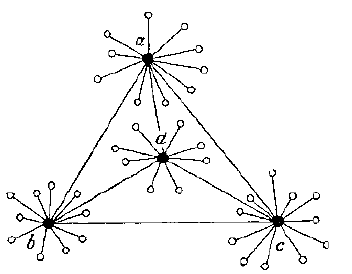
\includegraphics[width=0.5\textwidth]{example-imageю.png} % Replace with actual image path
    \caption{Рис. 4--6}
\end{figure}


\textbf{Лемма 1} Для двух графов $G$ и $H$
\[
\alpha(G \times H) \geq \alpha(G) \cdot \alpha(H)
\]

Действительно, если $S$ и $T$ — наибольшие внутренне устойчивые множества соответственно для $G$ и $H$, то декартово произведение $S \times T$ является внутренне устойчивым в графе $G \times H$, откуда
\[
\alpha(G \times H) \geq |S \times T| = |S| \cdot |T| = \alpha(G) \cdot \alpha(H)
\]

Эта лемма подсказывает нам следующее определение, назовем \emph{емкость} графа $G$ число
\[
\theta(G) = \sup_{n} \sqrt[n]{\alpha(G^n)}
\]

Имеем $\theta(G) \geq \alpha(G)$, мы собираемся показать, что почти всегда
\[
\theta(G) = \alpha(G)
\]

Между прочим, Шеннон установил, что граф $G$, изображенный на рис. 4-8, является единственным графом с числом вершин менее шести, для которого $\theta(G) \neq \alpha(G)$, фактически его емкость $\theta(G)$ не удалось определить, и известно лишь, что
\[
\forall \, 5 \leq \theta(G) \leq \frac{5}{2}
\]

Рассмотрим однозначное отображение $\sigma$ множества $X$ в себя, такое отображение называется \emph{сохраняющим}, если
\[
y \neq x, \, y \notin \Gamma(x) \Rightarrow \sigma(y) \neq \sigma(x), \, \sigma(y) \notin \Gamma(\sigma(x))
\]

Это отображение сохраняет свойство пары вершин "быть несмежными и различными".

\textbf{Лемма 2} Сохраняющее отображение $\sigma$ переводит внутренне устойчивое множество $S$ во внутренне устойчивое множество $\sigma(S)$, и при этом $|\sigma(S)| = |S|$.

В самом деле, ввиду однозначности отображения $\sigma$ имеем $|\sigma(S)| \leq |S|$, а так как $\sigma$ сохраняюще, то $|\sigma(S)| = |S|$.

\textbf{Лемма 3} Если множество $\sigma(X)$ внутренне устойчиво, то число внутренне устойчивости графа $G$ есть $\theta(G) = \alpha(G)$.

Действительно, раз $\sigma(X)$ внутренне устойчиво, то
\[
|\sigma(X)| \leq \max_{S} |S| = \alpha(G)
\]

С другой стороны, если $S_0$ — наибольшее внутренне устойчивое множество, то в силу леммы 2,

\[
|\sigma(X)| \geq |\sigma(S_0)| = |S_0| = \alpha(G),
\]

Отсюда

\[
\alpha(G) = |\sigma(X)|.
\]

\textbf{Теорема 7 (Шеннон)} \textit{Если хотя бы для одного из графов $G$ и $H$ существует сохранное отображение $\sigma$, переводящее множество вершин этого графа во внутренне устойчивое множество, то}

\[
\alpha(G \times H) = \alpha(G)\alpha(H).
\]

Достаточно показать, что $\alpha(G \times H) \leq \alpha(G)\alpha(H)$, пусть $\sigma$ — сохранное отображение для $G$, при котором $\sigma(X)$ внутренне устойчиво, и пусть $\sigma_0$ — отображение множества вершин графа $G \times H$ в себя, определенное следующим образом.

\[
\sigma_0(x, y) = (\sigma(x), y).
\]

Отображение $\sigma_0$ переводит две несмежные различные вершины $ξ = (x, y)$ и $ξ' = (x', y')$ в две несмежные различные вершины $(\sigma x, y)$ и $(\sigma x', y')$ и поэтому сохранно.

Если $S_0$ — наибольшее внутренне устойчивое множество графа $G \times H$, то $\alpha(G \times H) = |S_0| = |\sigma_0(S_0)|$ в силу леммы 2, распределим элементы $\sigma_0(S_0)$ по различным классам в зависимости от первой буквы каждого слова. Согласно лемме 3 получим: $|\sigma(X)| = \alpha(G)$ различных классов. Поскольку никакие два элемента из $\sigma_0(S_0)$ не смежны, каждый класс имеет самое большее $\alpha(H)$ элементов, значит

\[
\alpha(G \times H) = |\sigma_0(S_0)| \leq \alpha(G)\alpha(H).
\]

\textbf{Следствие} \textit{Если множество вершин графа $G$ при помощи сохранного отображения $\sigma$ можно перевести во внутренне устойчивое множество, то емкость этого графа совпадает с числом внутренней устойчивости.}

В самом деле,

\[
\alpha(G) \leq (\alpha(G))^2
\]

и

\[
\alpha(G \times G) \leq (\alpha(G))^3
\]

и т.д.,

отсюда

\[
\alpha(G) = \sup_n \sqrt[n]{\alpha(G^n)} = \alpha(G).
\]

%Внешнее устойчивое множество
\newpage\subsection{Внешнее устойчивое множество}
Граф $G = (X, \Gamma)$, множество $T \subseteq X$ внешне устойчиво, если для каждой вершины $x \notin T$ имеем $\Gamma_x \cap T \neq \varnothing$ (каждая вершина вне $T$ соединена с $T$). Если $\mathcal{T}$ — все внешне устойчивые множества, то $X \in \mathcal{T}$ и $T \in \mathcal{T} \quad A \supseteq T \Rightarrow A \in \mathcal{T}$.

\textbf{Число внешней устойчивости}
\[\beta(G) = \min_{T \in \mathcal{T}} |T|\] (минимальное внешне устойчивое множество).

\textbf{Алгоритм нахождения наименьшего внешне устойчивого множества}
\\1. Удаляем вершину $x$, если $\Delta x \subseteq \Delta y$ для $y \neq x$ (вершина $y$ заменяет $x$). Пример: удаляем $c, d, f$.
\\2. Если есть висячее ребро $(x, y)$, то $x \in T$. Пример: $a \in T$.
\\3. Исключаем $a$ и $\Delta a = \{\overline{a}, \overline{b}, \overline{c}\}$.
\\4. Повторяем шаги 1 и 2. Если граф неприводим, временно добавляем в $T$ вершину, например $b$.
\\5. Исключаем $b$ и $\Delta b = \{a, e, f\}$.
\\6. Упрощаем граф: исключаем $g$, так как $\Delta g \subseteq \Delta e = \{g\}$. Включаем $e$ в $T$, получаем $T = \{a, b, e\}$.

%Ядро графа
\newpage\subsection{Ядро графа}
Пусть $G = (X, \Gamma)$ — конечный или бесконечный граф. Множество $S \subseteq X$ называется \textit{ядром} графа, если $S$ устойчиво как внутренне, так и внешне, т.е. если

\begin{equation}
x \in S \Rightarrow \Gamma x \cap S = \varnothing,
\end{equation}

\begin{equation}
x \notin S \Rightarrow \Gamma x \cap S \neq \varnothing.
\end{equation}

Из условия (1) следует, что ядро $S$ не содержит петель. Из условия (2) — что $S$ содержит все такие вершины $x$, для которых $\Gamma x = \varnothing$. Пустое множество $\varnothing$ не может быть ядром.

\textbf{Теорема 1} \\
Если $S$ — ядро графа $(X, \Gamma)$, то множество $S$ — максимальное в семействе $\mathfrak{S}$ внутренне устойчивых множеств, т.е.
\[
A \in \mathfrak{S}, \, A \supseteq S \Rightarrow A = S
\]

\textbf{Теорема 2} \\
В симметрическом графе без петель каждое максимальное множество семейства $\mathfrak{S}$ внутренне устойчивых множеств представляет собой ядро.

\textbf{Следствие} \\
Симметрический граф без петель обладает ядром.

\textbf{Характеристическая функция} \\
Функция $\varphi_S(x)$ множества $S$ определяется как:

\[
\varphi_S(x) = 
\begin{cases} 
1, & \text{при } x \in S \\ 
0, & \text{при } x \notin S 
\end{cases}
\]

\textbf{Теорема 3} \\
Для того чтобы множество $S$ было ядром, необходимо и достаточно чтобы для характеристической функции $\varphi_S(x)$ выполнялось соотношение

\[
\varphi_S(x) = 1 - \max_{y \in \Gamma x} \varphi_S(y)
\]

\textbf{Теорема 4} \\
Прогрессивно конечный граф обладает ядром.

\textbf{Теорема Ричардсона} \\
Конечный граф, не содержащий контуров нечетной длины, обладает ядром.


%Игры на графе, игра НИМ
\newpage\subsection{Игры на графе, игра НИМ}

\textbf{Определение игры на графе}
Граф $(X, \Gamma)$ дает возможность определить некоторую игру двух игроков, которых мы назовем $(A)$ и $(B)$. Положениями этой игры служат вершины графа, начальная вершина $x_0$ выбирается жребием, и противники играют поочередно: сперва игрок $(A)$ выбирает вершину $x_1$ в множестве $\Gamma x_0$, затем $(B)$ выбирает вершину $x_2$ в множестве $\Gamma x_1$, после этого $(A)$ опять выбирает вершину $x_3$ в $\Gamma x_2$, и т.д. Если один из игроков выбрал вершину $x_n$, для которой $\Gamma x_n = \emptyset$, то партия оканчивается, игрок, выбравший вершину последним, выиграл, а его противник проиграл. Ясно, что если граф не является прогрессивно конечным (граф, в котором любая последовательность вершин заканчивается), то партия может никогда не окончиться.

\textbf{Игра НИМ}
В честь известного развлечения, которое здесь обобщено, будем описанную только что игру называть \textit{игрой Ним}, а определяющий ее граф обозначать через $(X, \Gamma)$; сейчас наша задача состоит в том, чтобы охарактеризовать выигрышные положения, т.е. те вершины графа, выбор которых обеспечивает выигрыш партии независимо от ответов противника.

\textbf{Теорема 1.} \textit{Если граф имеет ядро $S$ (множество вершин, из которых можно выиграть), и если один из игроков выбрал вершину в ядре, то этот выбор обеспечивает ему выигрыш или ничью.}

Действительно, если игрок $(A)$ выбрал вершину $x_1 \in S$, то либо $\Gamma x_1 = \emptyset$, и тогда он уже выиграл партию, либо его противник $(B)$ вынужден выбрать вершину $x_2 \in X \setminus S$, а значит, следующим ходом игрок $(A)$ может выбрать $x_3$ опять в $S$ и продолжать в том же духе. Если в какой-либо определенный момент один из игроков выбрал вершину $x_n$, для которой $\Gamma x_n = \emptyset$, то $x_n \in S$, и выигравшим партнером необходимо является $(A)$.

\textbf{Метод вычисления выигрышных позиций}
Основной метод для хорошего игрока состоит, следовательно, в вычислении какой-либо функции Гранди (функция, определяющая выигрышные позиции), если она существует, с помощью этой функции \( g(x) \) получаем ядро
\[
S = \{ x | g(x) = 0 \}
\]
рассматриваемого графа. Если начальная вершина \( x_0 \) такова, что \( g(x_0) = 0 \), то игрок (A) находится в критическом положении, ибо его противник может обеспечить себе выигрыш или ничью. Напротив, если \( g(x_0) \neq 0 \), то игрок (A) сам обеспечивает себе выигрыш или ничью, выбирая такую вершину \( x_1 \), что \( g(x_1) = 0 \).

\textbf{Следствие.} Если граф прогрессивно конечен, то существует одна и только одна функция Гранди \( g(x) \), каждый выбор такой вершины \( y \), для которой \( g(y) = 0 \), является выигрышным, а каждый выбор такой вершины \( z \), что \( g(z) \neq 0 \), — проигрышным. (Непосредственно)


%\subsection{Транспортные сети}
%\subsection{Теорема Кёнига-Холла}
%\subsection{Приложения к матрицам}
%\subsection{Бистохастические матрицы}
%\subsection{Теорема Биркгофа - фон Неймана}

\end{document}